\documentclass[xcolor=dvipsnames]{beamer}
% Sandpiles
\mode<presentation>
\usetheme{silab} 
\usecolortheme{silab}

\usepackage{listings}
\usepackage{pxfonts}

% Show Date in title
\def\showtitledate{}
%\def\fancystyle{}
%\def\showshorttitle{}


% Some color definitions
\definecolor{mygray}{gray}{.75}
\definecolor{titlegray}{gray}{.35}
\definecolor{lightgray}{gray}{.85}
\definecolor{topgray}{gray}{.85}
\definecolor{myblue}{rgb}{0.8, 0.85, 1}
\definecolor{topblue}{rgb}{0.68, 0.68, 0.88}
\definecolor{visblack}{rgb}{0.0, 0.0, 0.0}

% Boxes
\setbeamercolor{uppercol}{fg=black,bg=myblue}
\setbeamercolor{lowercol}{fg=black,bg=mygray}

\usepackage[english]{babel}
\usepackage[utf8]{inputenc}
\usepackage[T1]{fontenc}
\usepackage{graphicx}
\usepackage{amsmath,commath,amsfonts,amssymb,mathtools}
\usepackage{pgf}
\usepackage[autostyle=true]{csquotes}
\usepackage{IEEEtrantools}
\usepackage[varg]{txfonts}
\usepackage{hyperref}
\usepackage{xcolor}
\usepackage[table-format=1.4, separate-uncertainty=false]{siunitx}
\usepackage{fancyhdr}
\usepackage{colortbl}
\usepackage{geometry}
\usepackage{caption}
\usepackage{siunitx}
\usepackage{verbatim}
\usepackage{subfigure}
\usepackage{booktabs}
\usepackage{empheq}
\usepackage{animate}
\usepackage{float}
\usepackage{pdfpages}
\usepackage{multirow}
\usepackage{bigdelim}
\usepackage{floatflt}
\usepackage{scalerel}
\usepackage{tikz}
\graphicspath{{./pics/}{./gifs/}{../analysis/avalanche_formations/}{../analysis/moment_analysis/plots/}
              {../analysis/naive_fits/}{../report/gfx/}}
%\usepackage{ubonn-biblatex}
\usepackage[sorting=none, natbib=true, style=numeric]{biblatex}


\addto{\captionsenglish}{\renewcommand*{\figurename}{Fig.}}
\setbeamertemplate{caption}[numbered]

\newcommand*\widefbox[1]{\fbox{\hspace{2em}#1\hspace{2em}}}
\newcommand{\myitemsep}{\setlength\itemsep{0.33cm}}
\newcommand{\mysubitemsep}{\setlength\itemsep{0.22cm}}

\newcommand{\backupbegin}{
    \newcounter{finalframe}
    \setcounter{finalframe}{\value{framenumber}}
}
\newcommand{\backupend}{
    \setcounter{framenumber}{\value{finalframe}}
}

% Coding stuff
\lstset{language=python, numbers=left, numberstyle=\tiny, showstringspaces=false,
    aboveskip=10pt, frame=leftline}

% No stupid navigation bar
\beamertemplatenavigationsymbolsempty

\useinnertheme{rectangles}
%\setbeamertemplate{navigation symbols}{}

\title[Sandpiles]{Cellular Automata for Sandpiles}
\subtitle{An Example of Self-organized criticality}
\author[M. Frohne \& P. Wolf]{Markus Frohne\\ \texttt{\textcolor{gray}{markusfrohne@uni-bonn.de}}\\
        \vspace{0.33cm} Pascal Wolf\\ \texttt{\textcolor{gray}{pwolf@uni-bonn.de}}}
\date{March 15$^\text{th}$, 2018}

\addbibresource{../report/refs.bib}

\newcommand{\fplus}[1][black]{%
    \tikz\draw[#1,line width=2pt] (0,0) -- (0.25,0)(0.125,0.125) -- (0.125,-0.125);
}

\newcommand{\fminus}[1][black]{%
    \tikz\draw[#1,line width=2pt] (0,0) -- (0.25,0);
}

\renewcommand*{\thefootnote}{\fnsymbol{footnote}}

\begin{document}
    
    \begin{frame}
        \titlepage
    \end{frame}
    
    \begin{frame}[t]{Outline of talk}
        \begin{itemize}
            \myitemsep
            \item Motivation
            \item {Theory
                \vspace{0.22cm}
                \begin{itemize}
                    \mysubitemsep
                    \item[$\bullet$] Self-organized criticality (\textbf{SOC}) and Scale invariance
                    \item[$\bullet$] The \texttt{Bak-Tang-Wiesenfeld} (\textbf{BTW}) and Custom model
                \end{itemize}}
            \item {Simulations
                \vspace{0.22cm}
                \begin{itemize}
                    \mysubitemsep
                    \item[$\bullet$] Visualization of simulated data
                \end{itemize}}
            \item {Analysis
                \vspace{0.22cm}
                \begin{itemize}
                    \mysubitemsep
                    \item[$\bullet$] Methods
                    \item[$\bullet$] Results
                    \item[$\bullet$] Discussion \& Comparison
                \end{itemize}}
            \item Summary
        \end{itemize}
    \end{frame}
    
    {\usebackgroundtemplate%
        {%
            
\includegraphics[width=\paperwidth,height=\paperheight]{bkg1.pdf}%
        }
        \begin{frame}
            \centering \Huge \color{ublue} Motivation
            \thispagestyle{empty}
            \addtocounter{framenumber}{-1}
        \end{frame}
    }
    
    \begin{frame}[t]{Motivation}
        \begin{itemize}\myitemsep
            \item<1-> Critical phenomena are studied widely
            \item<2-> The Ising model% consists of a collective of magnetic moments represented by spins $\vec{s}$
                                 % on a lattice:
            \begin{itemize}\mysubitemsep
                \item[$\bullet$] Main tunable model parameter: temperature $T$
                \item[$\bullet$] Phase transition at critical temperature $T_{\mathrm{c}}$
                \item[$\bullet$] Cluster formation with characteristic properties (scale invariance!)
            \end{itemize}
        \end{itemize}
        \only<3->{\begin{figure}[htb]
            \centering
            \animategraphics[width=0.4\linewidth, loop, autoplay]{10}{ising-}{0}{199}
            \caption{Ising model cluster formation around the critical temperature.}
            \label{fig:ising}
        \end{figure}}
    \end{frame}

    \begin{frame}[t]{Motivation}
        \vspace{-1em}
        \begin{columns}[t]
            \begin{column}{0.6\linewidth}
                \begin{itemize}\myitemsep
                    \item<1-> Different types of critical phenomena
                        \begin{enumerate}\mysubitemsep
                            \item[$\bullet$] need tuning of parameter
                            \item[$\bullet$] don't need tuning of parameter \large ?
                        \end{enumerate}
                    \item<2-> Critical phenomena without tuning exist:\\
                          Examples from nature~\cite{Hergarten}
                            \begin{itemize}\mysubitemsep
                                \item[$\bullet$] landslides
                                \item[$\bullet$] earthquakes
                                \item[$\bullet$] seacoasts
                                \item[$\bullet$] forest fires
                                \item[$\bullet$] \textbf{sandpiles}
                            \end{itemize}
                    \item<4-> No tuning needed $\rightarrow$ \enquote{self-organized}\\
                              \makebox[\widthof{No tuning needed $\rightarrow$ \,\,}]{}criticality
                \end{itemize}
            \end{column}
            \begin{column}{0.4\linewidth}
                \only<3->{\begin{figure}[htb]
                    \centering
                    \includegraphics[width=0.8\linewidth]{landslide}
                    \caption{A rock landslide in Guerrero, Mexico.\\
                             \footnotesize from: Wikimedia Commons, \emph{File:Slide-guerrero1.JPG}}
                    \label{fig:}
                \end{figure}}
            \end{column}
        \end{columns}
    \end{frame}

    
    {\usebackgroundtemplate%
        {%
            
\includegraphics[width=\paperwidth,height=\paperheight]{bkg1.pdf}%
        }
        \begin{frame}
            \centering \Huge \color{ublue} Theory
            \thispagestyle{empty}
            \addtocounter{framenumber}{-1}
        \end{frame}
    }

    \begin{frame}[t]{Theory -- SOC and scale invariance}
        \begin{itemize}\myitemsep
            \item<1-> Some definitions:
                \begin{itemize}\mysubitemsep
                    \item[$\bullet$] \textbf{SOC system}:
                                     System that naturally evolves into a critical equilibrium state by itself
                                     without parameter tuning
                    \item[$\bullet$] \textbf{Scale invariance}:
                                     Dynamics of the considered system do not change under rescaling
                \end{itemize}\vspace{1em}
            \item<2> Every SOC system is believed to show scale invariance
                \begin{itemize}\mysubitemsep
                    \item[$\bullet$] Observables $\hat{Y}$ follow power law distribution:
                    \begin{align*}
                    P^{(Y)}(y) \propto y^{-\rho}
                    \end{align*}
                    \item[$\bullet$] Scaling factor $\lambda$ retains form of power law:
                    \begin{align*}
                    P^{(Y)}(\lambda y) \propto (\lambda y)^{-\rho} \propto y^{-\rho} \propto P^{(Y)}(y)
                    \end{align*}
                \end{itemize}
        \end{itemize}
    \end{frame}

    \begin{frame}[t]{Theory -- Scale invariance of sandpiles}
        \begin{itemize}\myitemsep
            \item Need observables\only<2->{:}
                \begin{itemize}\mysubitemsep
                    \item<2->[$\bullet$] Avalanche Area
                    \item<3->[$\bullet$] Avalanche Duration
                    \item<4->[$\bullet$] Avalanche Size
                \end{itemize}\vspace{1em}
            \item<5> Need distributions of observables:
                \begin{itemize}\mysubitemsep
                    \item[$\bullet$] Simulate sandpiles numerically
                    \item[$\bullet$] Use cellular automata:
                        \begin{itemize}\mysubitemsep
                            \item[$\nabla$] Iterative algorithm acting on a discrete lattice
                            \item[$\nabla$] Lattice sites are repeatedly updated\\
                                            depending on current lattice state
                        \end{itemize}
                \end{itemize}
        \end{itemize}
    \end{frame}
    
    \begin{frame}[t]{Theory -- Sandpile cellular automata}
        \begin{itemize}\myitemsep
            \item<1-> The \texttt{Bak-Tang-Wiesenfeld} (BTW) model
                \begin{itemize}\mysubitemsep
                    \item<2->[$\bullet$] First model studying SOC in sandpile dynamics
                    \item<2->[$\bullet$] Stores local slopes of the sandpile on a lattice
                    \item<2->[$\bullet$] \textbf{Driving}: add sand to the pile $\Rightarrow$ increase slope
                    \item<2->[$\bullet$] \textbf{Relaxation}: Redistribute grains if slope is too large
                                                              $\Rightarrow$ change slopes
                \end{itemize}
        \end{itemize}
        \only<3->{
        \begin{figure}[h]
            \captionsetup{width=0.9\textwidth}
            \centering
            \only<3>{
            \subfigure[BTW lattice]{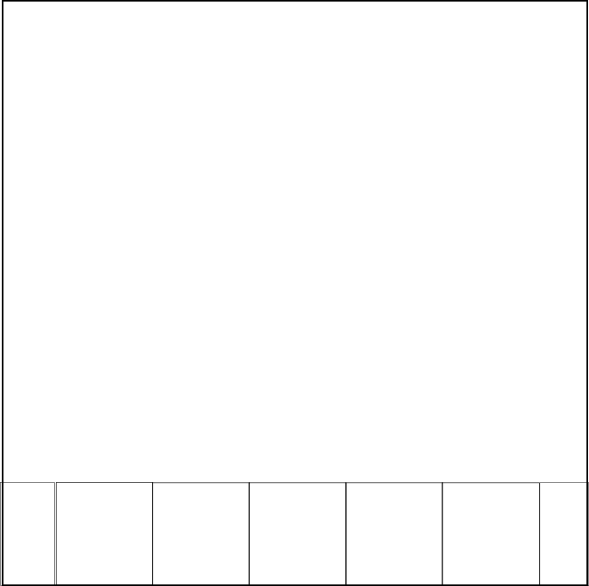
\includegraphics[width=0.2\textwidth]{drivingBTW0}}
            \subfigure[Sand grains]{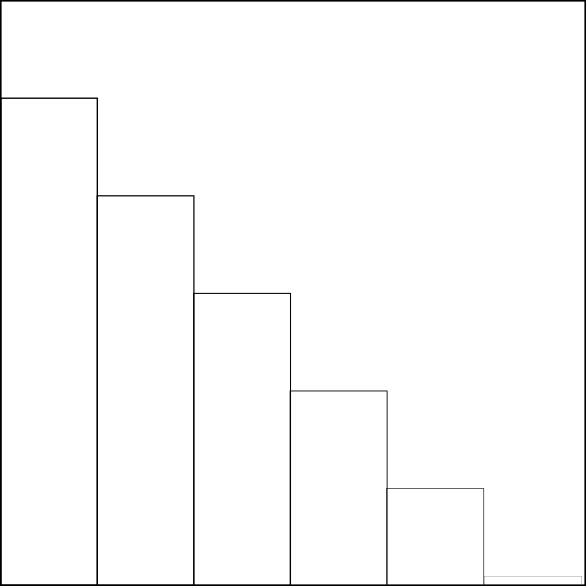
\includegraphics[width=0.2\textwidth]{drivingNonCons0}}}
            \only<4>{
            \subfigure[BTW lattice]{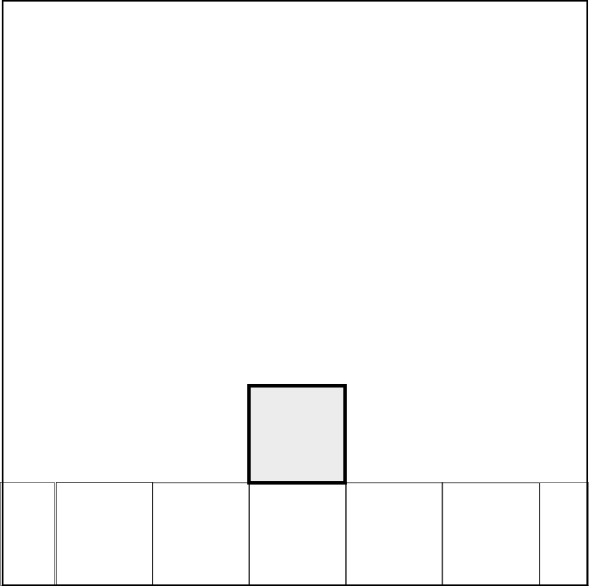
\includegraphics[width=0.2\textwidth]{drivingBTW1}}
            \subfigure[Sand grains]{
\includegraphics[width=0.2\textwidth]{drivingNonCons}}}
            \only<5>{
            \subfigure[BTW lattice]{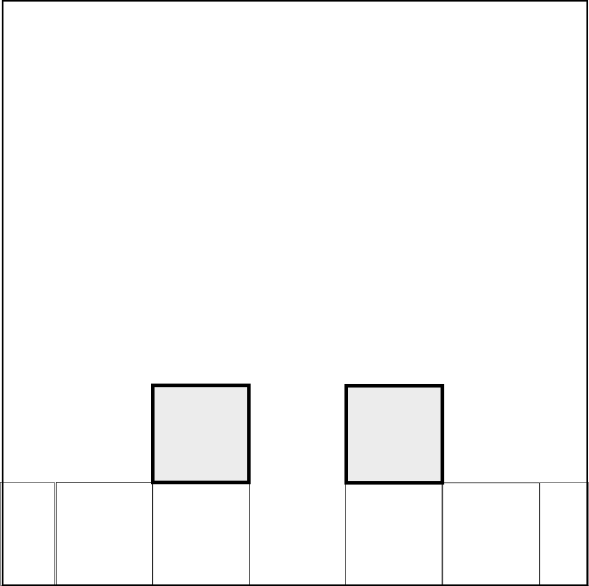
\includegraphics[width=0.2\textwidth]{drivingBTW2}}
            \subfigure[Sand grains]{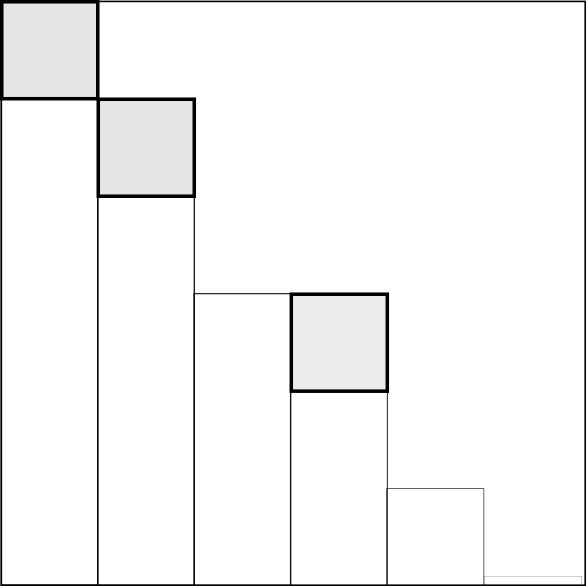
\includegraphics[width=0.2\textwidth]{drivingNonCons1}}}
            \only<6>{
            \subfigure[BTW lattice]{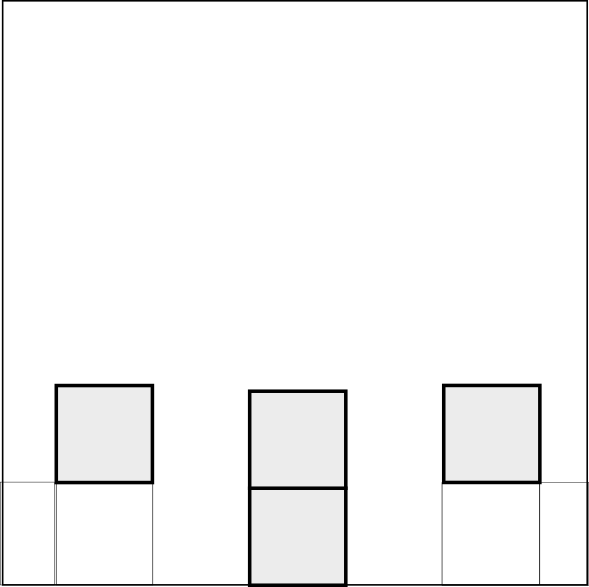
\includegraphics[width=0.2\textwidth]{drivingBTW3}}
            \subfigure[Sand grains]{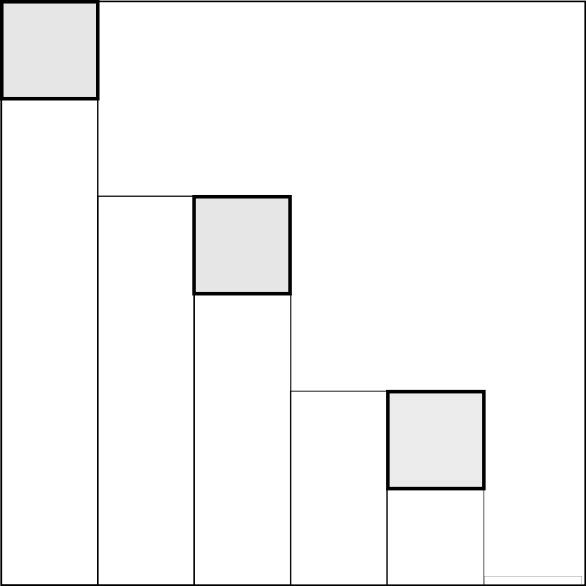
\includegraphics[width=0.2\textwidth]{drivingNonCons2}}}
            \only<7>{
            \subfigure[BTW lattice]{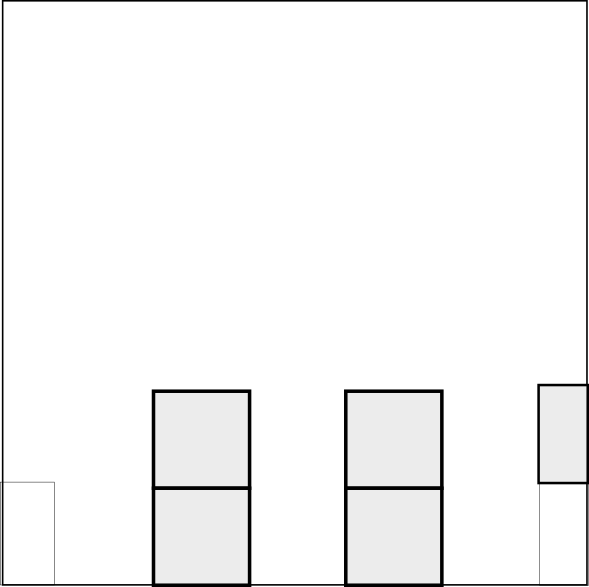
\includegraphics[width=0.2\textwidth]{drivingBTW4}}
            \subfigure[Sand grains]{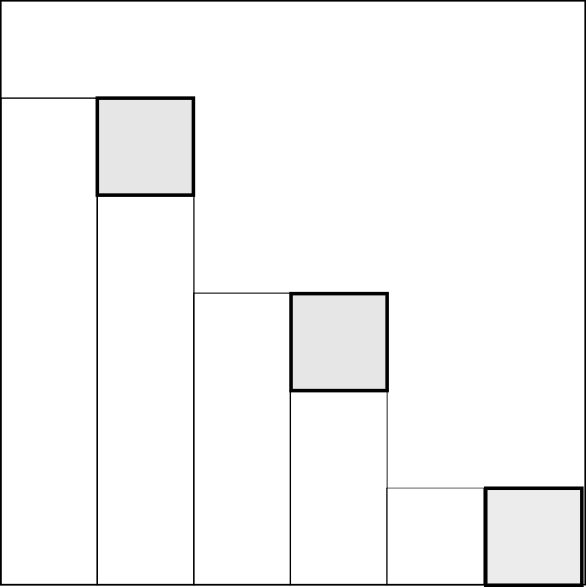
\includegraphics[width=0.2\textwidth]{drivingNonCons3}}}
            \only<8>{
            \subfigure[BTW lattice]{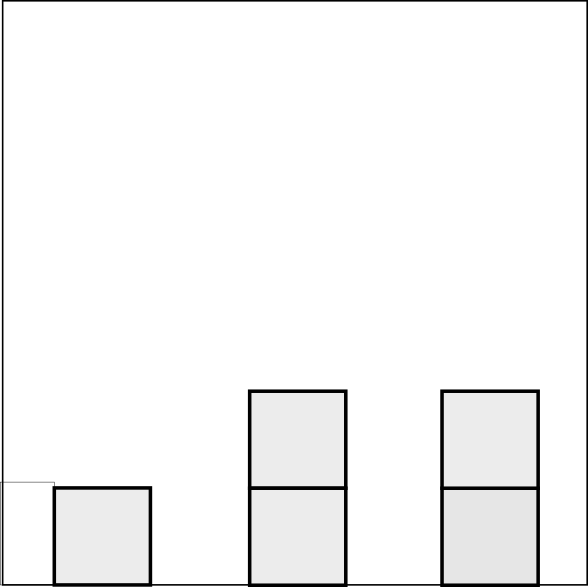
\includegraphics[width=0.2\textwidth]{drivingBTW5}}
            \subfigure[Sand grains]{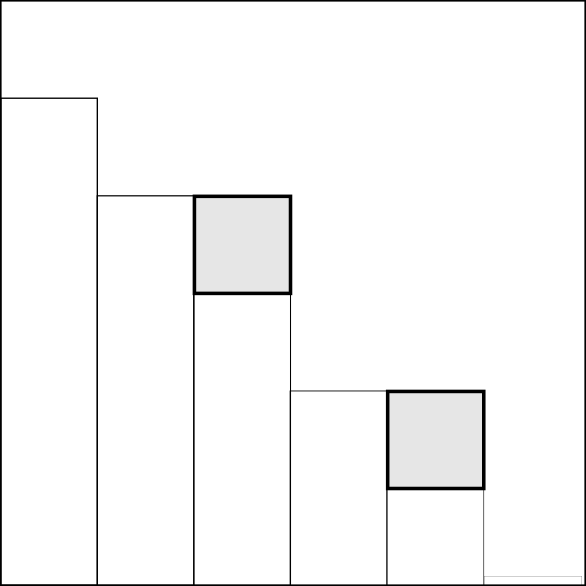
\includegraphics[width=0.2\textwidth]{drivingNonCons4}}}
            \only<9>{
            \subfigure[BTW lattice]{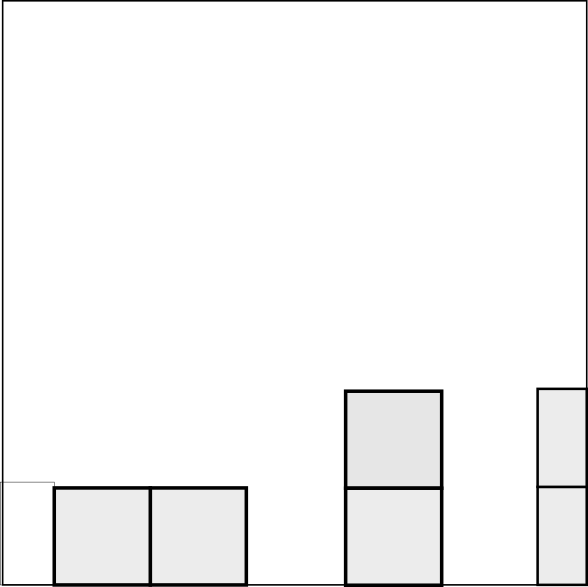
\includegraphics[width=0.2\textwidth]{drivingBTW6}}
            \subfigure[Sand grains]{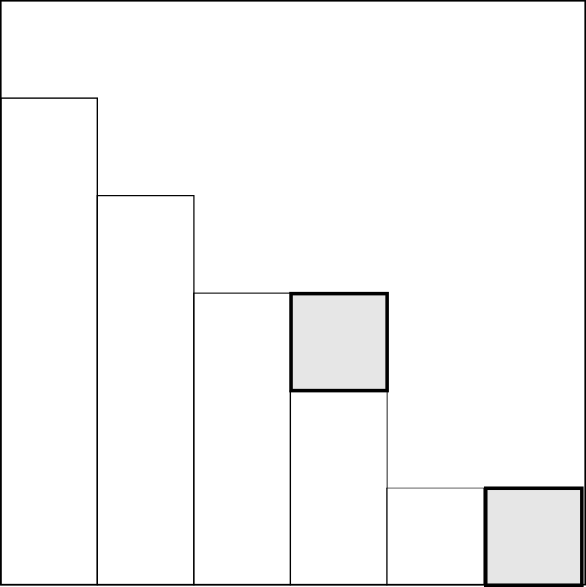
\includegraphics[width=0.2\textwidth]{drivingNonCons5}}}
            \only<10>{
            \subfigure[BTW lattice]{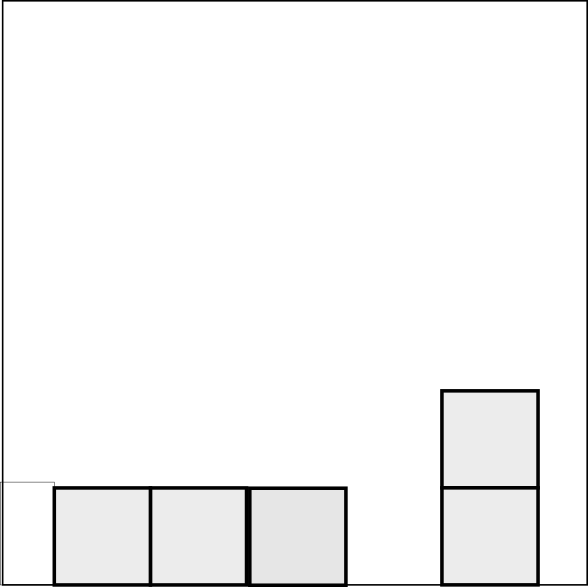
\includegraphics[width=0.2\textwidth]{drivingBTW7}}
            \subfigure[Sand grains]{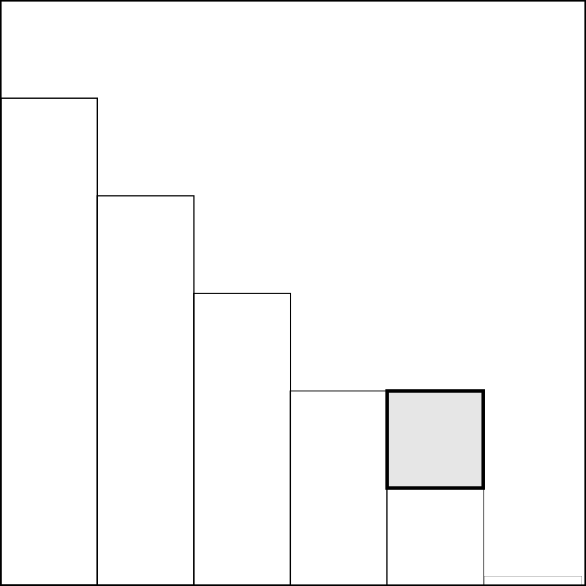
\includegraphics[width=0.2\textwidth]{drivingNonCons6}}}
            \only<11>{
            \subfigure[BTW lattice]{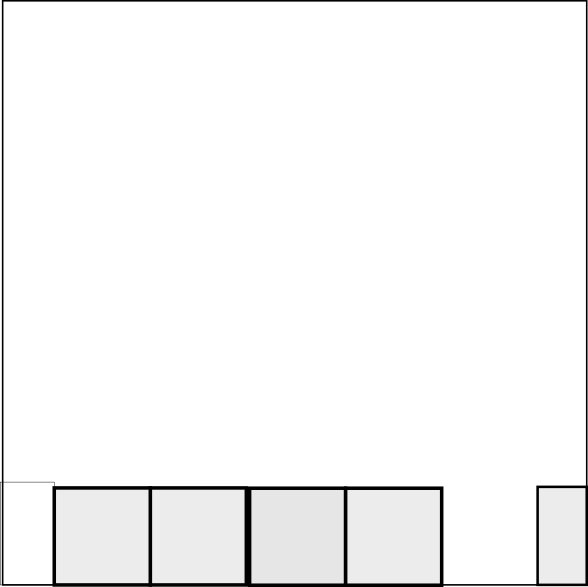
\includegraphics[width=0.2\textwidth]{drivingBTW8}}
            \subfigure[Sand grains]{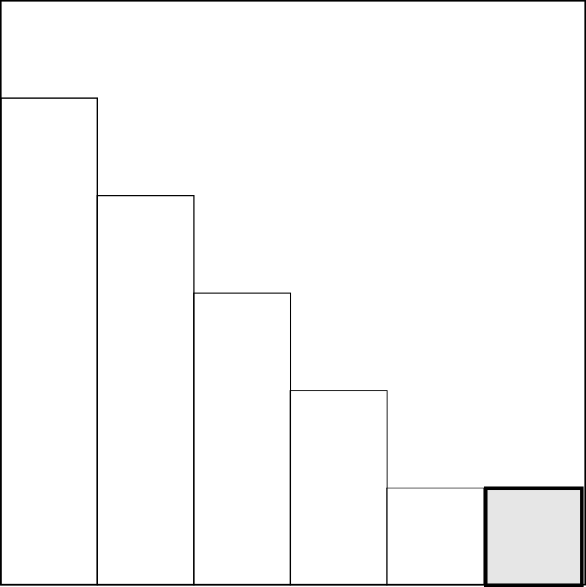
\includegraphics[width=0.2\textwidth]{drivingNonCons7}}}
            \only<12>{
            \subfigure[BTW lattice]{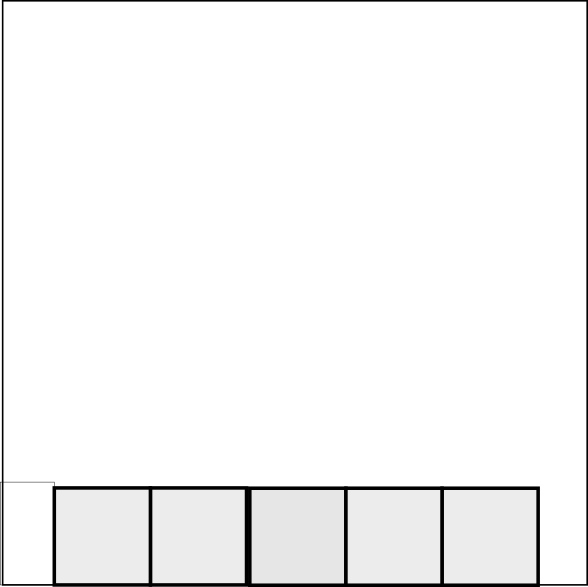
\includegraphics[width=0.2\textwidth]{drivingBTW9}}
            \subfigure[Sand grains]{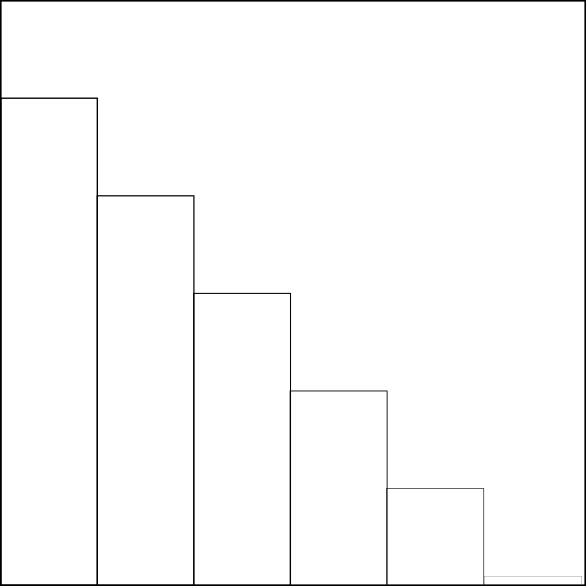
\includegraphics[width=0.2\textwidth]{drivingNonCons0}}}
            \only<13>{
            \subfigure[BTW lattice]{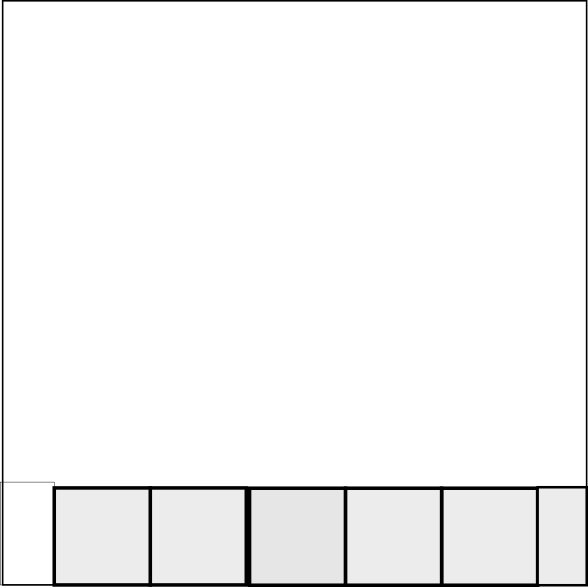
\includegraphics[width=0.2\textwidth]{drivingBTW10}}
            \subfigure[Sand grains]{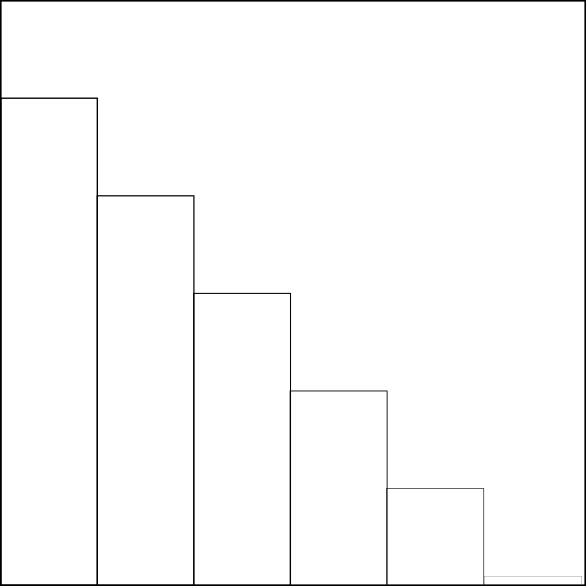
\includegraphics[width=0.2\textwidth]{drivingNonCons0}}}
            \caption{Driving and relaxation of BTW lattice.}
        \end{figure}
        }
    \end{frame}

    \begin{frame}[t]{Theory -- Sandpile cellular automata}
        \begin{itemize}\myitemsep
            \item<1-> The custom model
                \begin{itemize}\mysubitemsep
                    \item<2->[$\bullet$] Different approach
                    \item<2->[$\bullet$] Store local sandpile \emph{heights} instead of \emph{slopes} on the lattice
                    \item<2->[$\bullet$] \textbf{Driving}: add one grain of sand to the random site instead of the
                                                whole upper hillside
                    \item<2->[$\bullet$] \textbf{Relaxation}: Redistribute grains if slope is too large and
                                                   consider direction of slope
                \end{itemize}
            \only<3->{
            \begin{figure}[h]
                \captionsetup{width=0.9\textwidth}
                \centering
                \subfigure[Non-con\-ser\-va\-ti\-ve]{
\includegraphics[width=0.15\textwidth]{drivingNonCons}}
                \hspace{1em}
                \subfigure[Conservative]{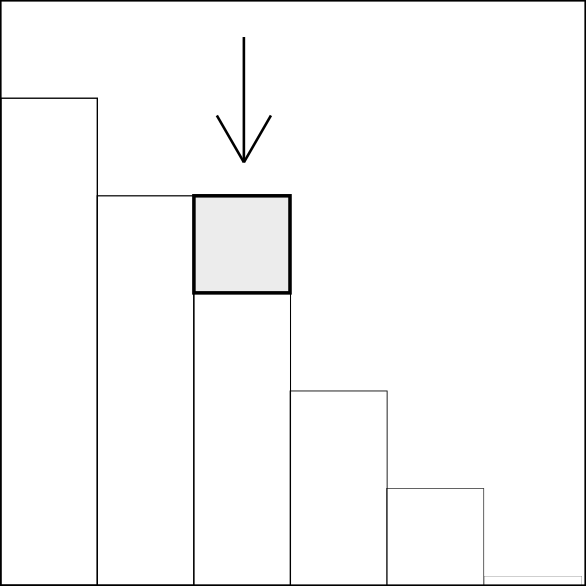
\includegraphics[width=0.15\textwidth]{drivingCons}}
                \caption{Conservative and non-conservative driving.}
            \end{figure}
            }
        \end{itemize}
    \end{frame}

    {\usebackgroundtemplate%
        {%
            
\includegraphics[width=\paperwidth,height=\paperheight]{bkg1.pdf}%
        }
        \begin{frame}
            \centering \Huge \color{ublue} Simulations \\ \Large Visualization of data
            \thispagestyle{empty}
            \addtocounter{framenumber}{-1}
        \end{frame}
    }
    
    \begin{frame}[t]{Sandpile dynamics -- Avalanche evolution}
        \begin{figure}[h]
            \captionsetup{width=0.9\textwidth}
            \centering
            \only<1>{
            \subfigure[BTW model]{\animategraphics[width=0.475\textwidth, loop, autoplay]{10}{btw_center_}{1}{250}}
            \subfigure[Custom model]{\animategraphics[width=0.475\textwidth, loop, autoplay]{10}{custom_center_}{1}{250}}
            \caption{Avalanche evolution in a 2D sandbox of length 50 (\textbf{center} drives)}}
            \only<2>{
            \subfigure[BTW model]{\animategraphics[width=0.475\textwidth, loop, autoplay]{10}{btw_random_}{1}{250}}
            \subfigure[Custom model]{\animategraphics[width=0.475\textwidth, loop, autoplay]{10}{custom_random_}{1}{250}}
            \caption{Avalanche evolution in a 2D sandbox of length 50 (\textbf{random} drives)}}
        \end{figure}
    \end{frame}
    
    \begin{frame}[t]{Sandpile dynamics -- Avalanche formations}
        \begin{figure}[h]
            \captionsetup{width=0.9\textwidth}
            \begin{center}
                \only<1>{
                \subfigure[2D]{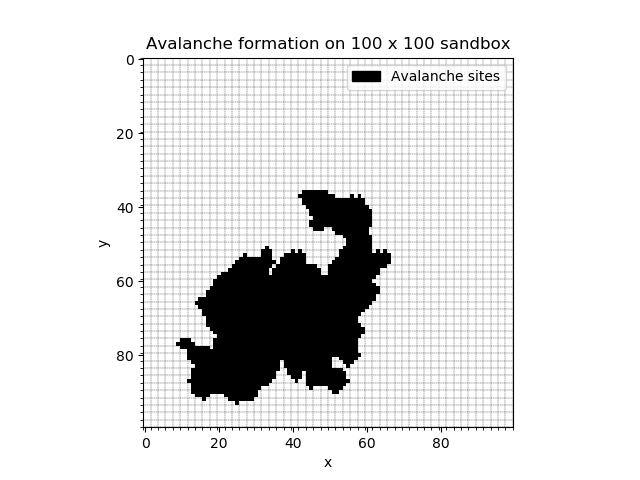
\includegraphics[width=0.475\textwidth]{Avalanche_2d_btw_1.png}}
                \subfigure[3D]{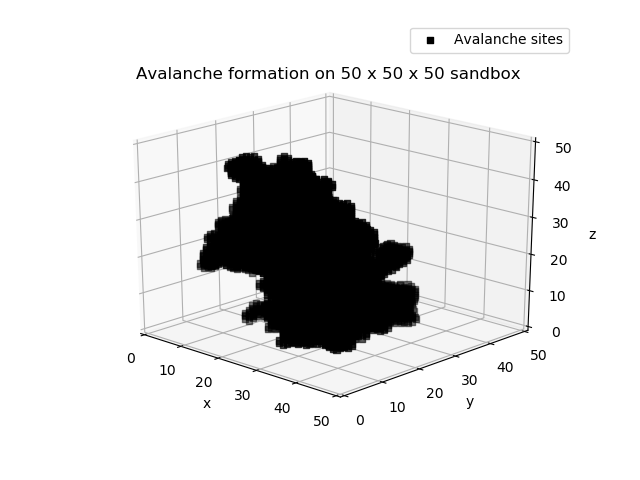
\includegraphics[width=0.475\textwidth]{Avalanche_3d_btw_6.png}}
                \caption{Avalanche formation in the BTW model.}}
                \only<2>{
                \subfigure[2 D]{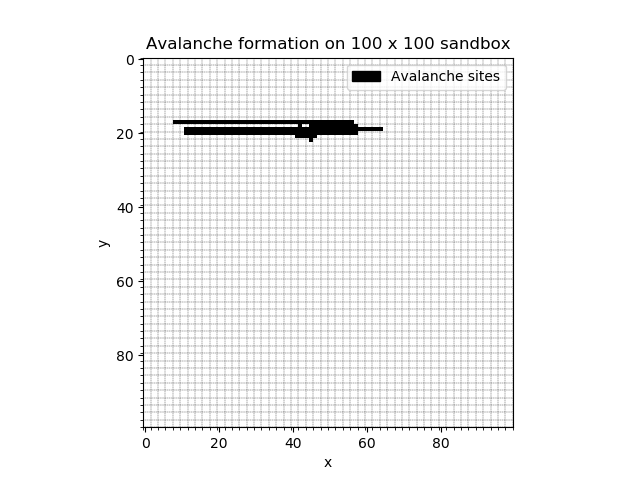
\includegraphics[width=0.475\textwidth]{Avalanche_2d_custom_11.png}}
                \subfigure[3 D]{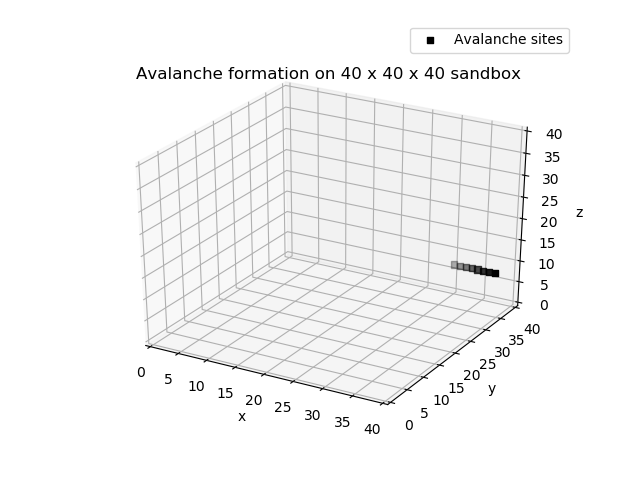
\includegraphics[width=0.475\textwidth]{Avalanche_3d_custom_4.png}}
                \caption{Avalanche formation in the custom model.}}
            \end{center}
        \end{figure}
    \end{frame}
    
    
    {\usebackgroundtemplate%
        {%
            
\includegraphics[width=\paperwidth,height=\paperheight]{bkg1.pdf}%
        }
        \begin{frame}
            \centering \Huge \color{ublue} Analysis
            \thispagestyle{empty}
            \addtocounter{framenumber}{-1}
        \end{frame}
    }
    
    \begin{frame}[t]{Analysis method -- Naive fit}
    	\begin{itemize}
    		\item {Initial method: straight line fit of power-law scaling behavior:
    			\begin{align*}
    			P^{(Y)}(y) \propto y^{-\rho}
    			\end{align*}}
    	\end{itemize}
    	\begin{minipage}[l]{0.5\textwidth}
    		\begin{itemize}
    			\item<2-> {$P^{(Y)}(y)$ deviates from linear trend due to e.g \textit{finite size effects}
    				\begin{itemize}
    					\item[$\bullet$] Straight line fit not sufficient to determine scaling exponents
    					\item[$\bullet$] No reasonable estimation of uncertainties on scaling exponents possible 
    				\end{itemize}}
    			\item<2->[$\Rightarrow$] More sophisticated approach: so-called \textit{moment analysis}
    		\end{itemize}
    	\end{minipage}
    	\begin{minipage}[r]{0.475\textwidth}
    		%\begin{figure}[h]
    			%\captionsetup{width=\textwidth}
    			\centering
    			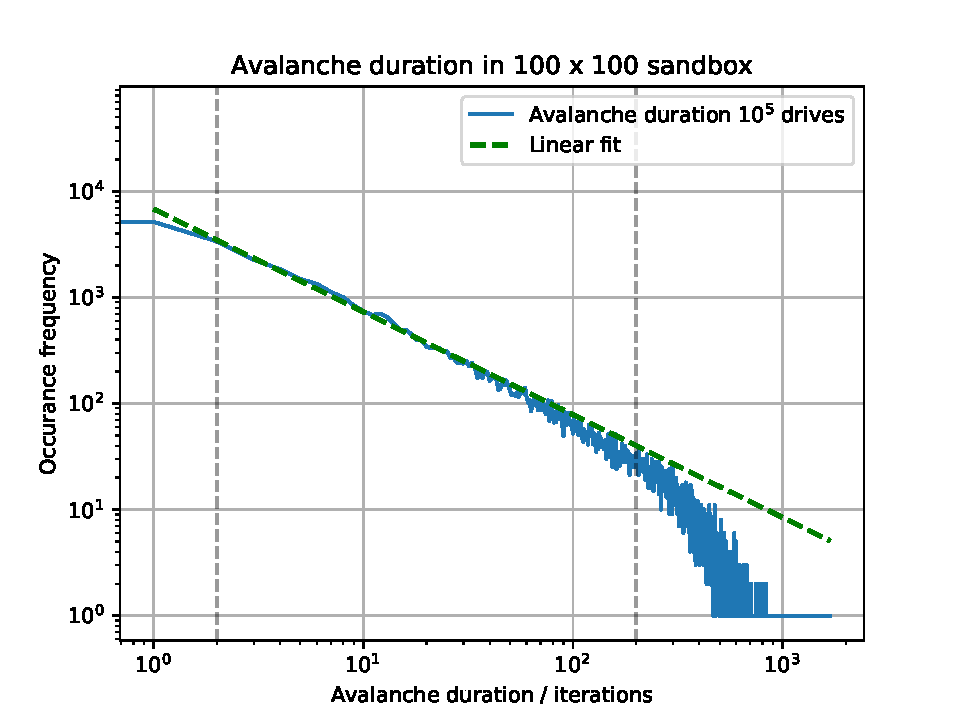
\includegraphics[width=\textwidth]{naive_fit.pdf}
    			%\caption{Power law scaling behavior of avalanche duration of the BTW model.}
    		%\end{figure}
    	\end{minipage}
    \end{frame}
    
    \begin{frame}[t]{Analysis method -- Moment analysis}
        \begin{itemize}
            \myitemsep
            \item {Define the so-called $n^{\mathrm{th}}$ \textit{moment} of the observable $\hat{Y}$ by
                \begin{align*}
                \left\langle y^n \right\rangle = \int_{0}^{\infty} dy\ y^n P^{(Y)}(y) \quad \text{where}
                \quad P^{(Y)}\equiv \text{PDF of}\ \hat{Y}
                \end{align*}
            }
            \item {For $L \to \infty$ (or approx. $L\gg 1$) the following relation holds:
                \begin{align*}
                \left\langle y^n \right\rangle \propto L^{K\left(1 + n - \rho \right)} \qquad \text{with}
                                                                \qquad K\left(1 + n - \rho \right) \equiv \sigma_n 
                \end{align*}
                where $K,\ \rho$ is the set of scaling exponents of the observable $\hat{Y}$. Taking the logarithm,
                this relation exhibits a linear trend with slope $\sigma_n$.
            }
            \item {Determination of the set of scaling exponents $K,\ \rho$ via linear fit of the $1^{\text{st}}$ and
                   $2^{\text{nd}}$ moments, yielding $\sigma_1$ and $\sigma_2$, like:
                \begin{align*}
                K = \sigma_2 - \sigma_1 \quad , \quad \rho = \frac{2\sigma_2 - 3\sigma_1}{\sigma_2 - \sigma_1} 
                \end{align*} 
            }
        \end{itemize}
    \end{frame}
    
    \begin{frame}[t]{Analysis method -- Moment analysis}
        \begin{itemize}
            \myitemsep
            \item {General approach of moment analysis:
                \begin{itemize}
                    \mysubitemsep
                    \item[$\bullet$] Simulate $R$ samples for $N$ lattice sizes $L_N$, record PDF of observables and
                                     calculate $\left\langle y^1 \right\rangle,\ \left\langle y^2 \right\rangle$
                    \item[$\bullet$] Draw \textit{random} bootstrap sample from $\left\langle y^1 \right\rangle_R,
                                     \ \left\langle y^2 \right\rangle_R$ for each $L_N$
                    \item[$\bullet$] Calculate covariance matrix for each bootstrap (\textbf{double bootstrap})
                    \item[$\bullet$] Linear fit within each bootstrap sample to calculate and store $K,\ \rho$
                    \item[$\bullet$] $K,\ \rho = \left\langle K, \rho \right\rangle_{\mathrm{bootstraps}}$ and estimate
                                     uncertainty by $\sigma (K,\ \rho)_{\mathrm{bootstraps}}$
                \end{itemize}
            }
            \item[$\Rightarrow$] {Actual numbers for analysis in 2 and 3 dimensions:
                \begin{itemize}
                    \mysubitemsep
                    \item[$\bullet$] $R = 10$
                    \item[$\bullet$] $N = R$ with $L_N \in \{10, 20, 30, 40, 50, 60, 70, 80, 90, 100\}$
                \end{itemize}
            }
        \end{itemize}
    \end{frame}
    
    \begin{frame}[t]{Analysis method -- Moment analysis}
        \begin{figure}[htp]
            \centering
            \only<1>{
            \subfigure[BTW]{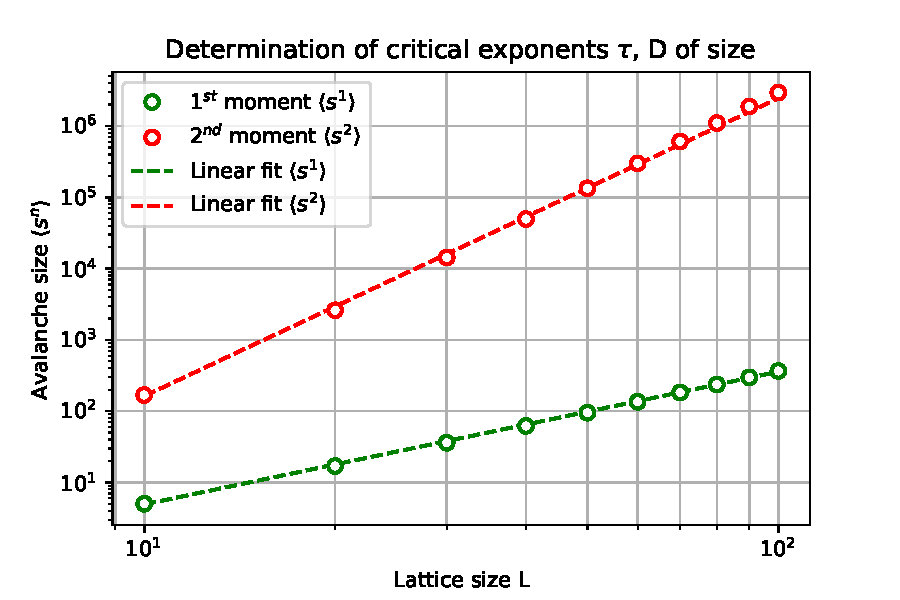
\includegraphics[width=0.475\textwidth]{moment_analysis_size_2d_btw_fit.pdf}}
            \subfigure[Custom]{\includegraphics[width=0.475\textwidth]{{moment_analysis_size_2d_custom_crit_%
                                                                        slope_7_fit.pdf}}}
            \caption{$1^{\mathrm{st}}$ and $2^{\mathrm{nd}}$ moments of one \textit{random} bootstrap sample for
                     avalanche \textbf{size} and overall best linear fit in 2D.}
            }
%            \only<2>{
%            \subfigure[BTW]{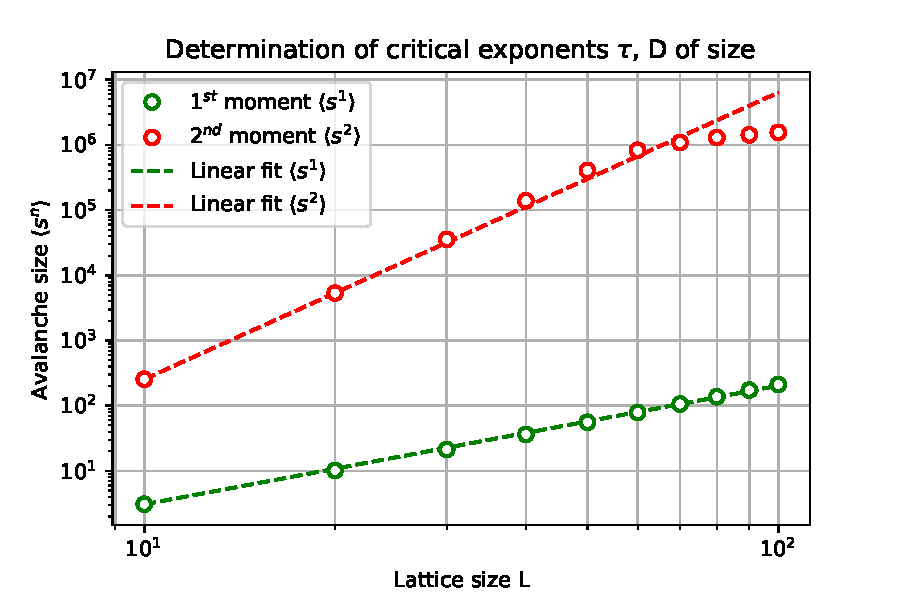
\includegraphics[width=0.475\textwidth]{moment_analysis_size_3d_btw_fit.pdf}}
%            \subfigure[Custom]{\includegraphics[width=0.475\textwidth]{{moment_analysis_size_3d_custom_crit_slope_%
%                                                                        5_fit.pdf}}}
%            \caption{$1^{\mathrm{st}}$ and $2^{\mathrm{nd}}$ moments of one \textit{random} bootstrap sample for
%                     avalanche \textbf{size} and overall best linear fit in 3D.}
%            }
        \end{figure}
    \end{frame}
    
    \begin{frame}[t]{Analysis results -- Moment analysis}
        \renewcommand{\arraystretch}{1.15}
        \begin{table}[htb]
            \centering
            \begin{tabular}{llSScSScSS}
            \toprule
            & \multirow{2}{*}{Model} & \multicolumn{2}{c}{Size} && \multicolumn{2}{c}{Duration} &&
                                                                   \multicolumn{2}{c}{Area} \\
            \cmidrule{3-4} \cmidrule{6-7} \cmidrule{9-10}
            && {$\tau$} & {$D$} && {$\alpha$} & {$Z$} && {$\kappa$} & {$T$} \\
            \cmidrule{2-10}
            \cmidrule{2-10}
            \hspace{-15px}\ldelim\lbrace{3}{0mm}[$2$D] &
            $\mathrm{BTW}$ & 1.19(9) & 2.3(2) && 1.21(2) & 1.34(3) && 1.23(7) & 1.9(2) \\
            & $\mathrm{CST}_{\mathrm{C}5}$ & 1.3(2) & 1.6(2) && 1.2(2) & 0.7(2) && 1.3(2) & 0.8(2) \\
            & $\mathrm{CST}_{\mathrm{C}7}$ & 1.4(2) & 1.6(4) && 1.3(1) & 0.81(8) && 1.4(1) & 1.0(1) \\
            \midrule
            \hspace{-15px}\ldelim\lbrace{2}{0mm}[$3$D] &
            $\mathrm{BTW}$ & 1.3(1) & 2.5(3) && 1.45(3) & 1.41(6) && 1.4(3) & 2.6(7) \\
            & $\mathrm{CST}_{\mathrm{C}5}$\footnote{No bootstrap fitting due to too few simulated samples} & 1.23(1) &
              1.99(2) && 1.29(1) & 1.17(1) && 1.29(1) & 1.43(1)\vspace{2px}\\
            \bottomrule
            \end{tabular}
            \caption{Scaling exponents for avalanche size, duration and area.}
            \label{tab:scalingExp}
        \end{table}
    \end{frame}
    
    \begin{frame}[t]{Analysis discussion -- Scaling exponents}
    	\only<1-3>{
    	\begin{itemize}
    		\myitemsep
    		\item<1-> {Comparison of results to literature possible, but:
	    		\begin{itemize}
	    			\item<2->[$\bullet$] Many different literature values of scaling exponents from various papers from
                                         the early 90's until today
	    			\item<2->[$\bullet$] Many different models used (\textbf{Abelian BTW}, Non-abelian BTW, etc.)
	    			\item<2->[$\bullet$] Usually only the sets $\tau,\ D$ and $\alpha,\ Z$ are stated
	    		\end{itemize}} 
    		\item<3> Generally, scaling exponents should satisfy $\tau, \alpha \ge 1$ for the BTW model
    		\item<3> Example in 2D: $\tau = \SI{1.2(1)}{},\ \alpha =\SI{1.16(3)}{}$ from \cite{SOC-book} coincide with
                     our simulations $\tau = \SI{1.19(9)}{},\ \alpha =\SI{1.21(2)}{}$.
    		\item<3> Scaling exponents of the BTW model determined in this project generally coincide with most of the
                     BTW literature values within their $\sigma$
    	\end{itemize}
    	}
    	\only<4>{
    	\begin{itemize}
    		\myitemsep
    		\item {Custom model partially deviates from BTW model: This is most prominent in the dimension exponents e.g.
                   of the avalanche area:
    			\begin{itemize}
    				\mysubitemsep
    				\item[$\bullet$] 2D area dimension exponent $T_{\mathrm{BTW}} = \SI{1.9(2)}{}$ vs.
                                     $T_{\mathrm{CST}} = \SI{1.0(1)}{}$ 
    				\item[$\Rightarrow$] {Custom avalanches are mostly 1 dimensional; That's also what we see:
    					\begin{figure}[h]
    						\centering
    						\subfigure[BTW 2D]{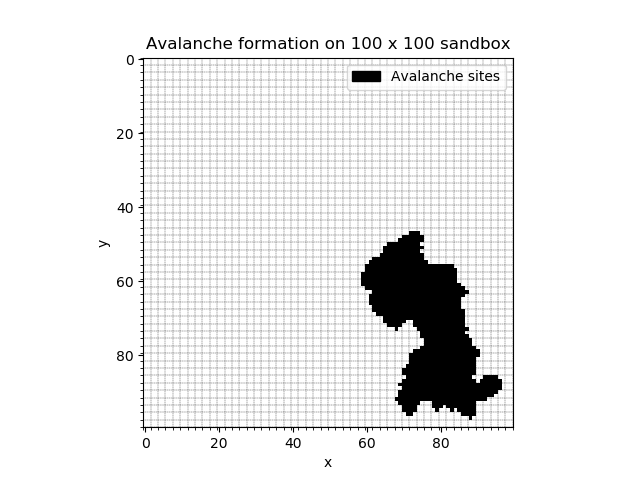
\includegraphics[width=0.275\textwidth]{Avalanche_2d_btw_3.png}}
    						\subfigure[CST 2D]{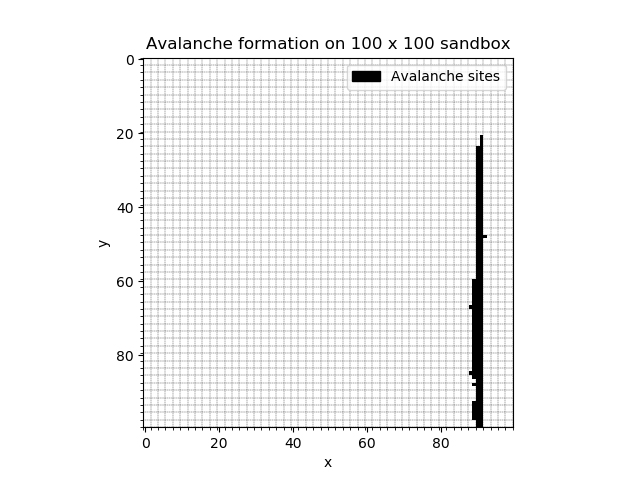
\includegraphics[width=0.275\textwidth]{Avalanche_2d_custom_1.png}}
    					\end{figure}
    					}
    			\end{itemize}}
   			\item Scaling exponents $\tau, \alpha$ of the custom model coincide with BTW
   		\end{itemize}
    	}
    \end{frame}
    
    \begin{frame}[t]{Analysis discussion -- Issues}
    	\begin{overlayarea}{\textwidth}{\textheight}
    	$\Rightarrow$ The main issue is the lack of computational resources: Inherits several consequences:\\\vspace{1cm}
    	\begin{minipage}[l]{0.585\textwidth}
    		\begin{itemize}
    			\only<1>{
    			\item Deviation from linear trend of $2^{\mathrm{nd}}$ moment for large lattices $L\ge 80$ in 3D:
    			\item[$\Rightarrow$] \# of drives of the simulation $<$ \# lattice sites: Not sufficient
    			\item[$\Rightarrow$] 1 simulation of $100^3$ lattice, $10^5$ drives $\approx$ \textbf{28 hours}
	    		}
	    		\only<2>{
    			\item Only samples for $L \le 40$ for custom model in 3D:
    			\item[$\Rightarrow$] Bootstrap fitting failed, external fitting library used
    			\item[$\Rightarrow$] No reliable estimation of uncertainty possible 
	    		}
	    		\only<3>{
    			\item 10 samples for each lattice size $L_N$ already very few:
    			\item[$\Rightarrow$] Double bootstrap needed
    			\item[$\Rightarrow$] Many bootstrap samples need to be drawn
	    		}
    		\end{itemize}
    	\end{minipage}
    	\begin{minipage}[r]{0.4\textwidth}
    		\centering
    		\only<1>{
    		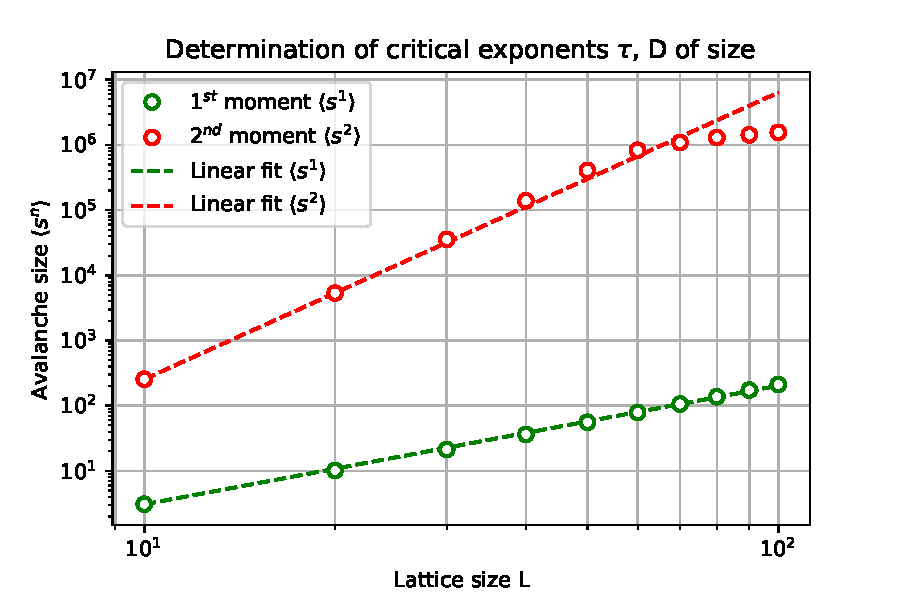
\includegraphics[width=\textwidth]{moment_analysis_size_3d_btw_fit.pdf}
	    	}
	    	\only<2>{
	    	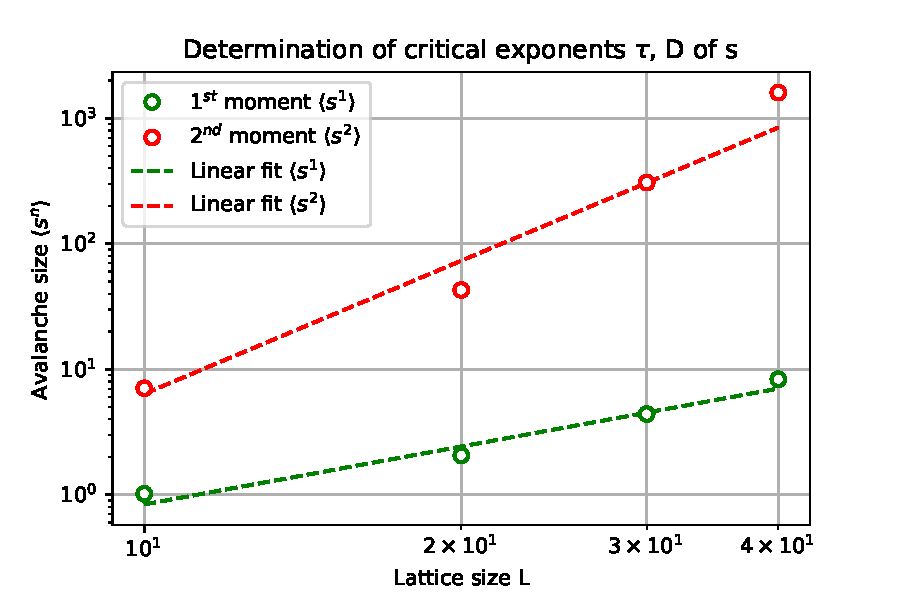
\includegraphics[width=\textwidth]{moment_analysis_size_3d_custom_crit_slope_5_fit.pdf}
	    	}
   		\end{minipage}
	   	\end{overlayarea}
   	\end{frame}
   	
   	\begin{frame}[t]{Summary and Conclusion}
   		\only<1>{
   		Within this project:\\
   		\begin{itemize}
   			\item {Two models of cellular automata for sandpile dynamics have been implemented
	   			\begin{itemize}
	   				\item[$\bullet$] The BTW model
	   				\item[$\bullet$] A custom model
	   			\end{itemize}
	   			}
	   		\item The characteristics, namely their sets of critical scaling exponents, have been determined  
   			\item The statistics were gathered for 2 and 3 dimensional lattices
   			\item The obtained results coincide with most of the values given in the literature
   		\end{itemize}
   		}
   		\only<2>{
		Conclusions:\\
		\begin{itemize}
			\item {More computational recourses would improve results:
				\begin{itemize}
					\item[$\bullet$] Simulate more samples and increase number of total drives
					\item[$\bullet$] Go to higher dimensions and lattice sites
				\end{itemize}
			}
			\item More detailed look / more configurations of the custom model would be interesting 
		\end{itemize}
		} 
   	\end{frame}
	
	{\usebackgroundtemplate%
		{%
			
\includegraphics[width=\paperwidth,height=\paperheight]{bkg1.pdf}%
		}
		\begin{frame}
			\centering \Huge \color{ublue} Thank you!% for your attention!
			\thispagestyle{empty}
			\addtocounter{framenumber}{-1}
		\end{frame}
	}
	   	
   	\begin{frame}[allowframebreaks]{Bibliography}
   		\printbibliography
   	\end{frame}
   	
   	{\usebackgroundtemplate%
   		{%
   			
\includegraphics[width=\paperwidth,height=\paperheight]{bkg1.pdf}%
   		}
   		\begin{frame}
   			\centering \Huge \color{ublue} Backup slides
   			\thispagestyle{empty}
   			\addtocounter{framenumber}{-1}
   		\end{frame}
   	}
   	
   	\backupbegin
   	
   	\begin{frame}[t]{Literature values}
   		\begin{minipage}[l]{0.3\textwidth}
   			\captionof{figure}{Literature values from various papers gathered in \cite{SOC-book}}
   		\end{minipage}
   		\begin{minipage}[r]{0.65\textwidth}
   			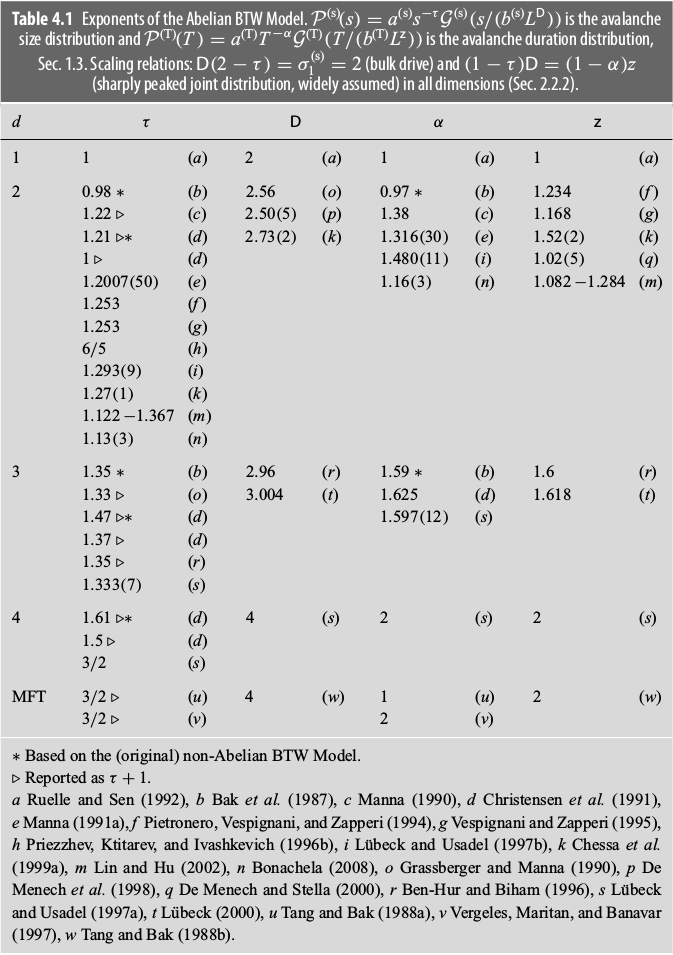
\includegraphics[height=0.85\textheight]{literature.png}
   		\end{minipage}
   	\end{frame}
   	\backupend

\end{document}
